%qqqqqqqqqqqqqqqqqqqqqqqqqqqqqqqqqqqqqqqqqqqqqqqqqqqqqqqqqqqqqqqqqqqqqqqqq
%Quote
\begin{savequote}[50mm]
‘‘El cosmos es todo lo que es, todo lo que fue y todo lo que será. Nuestras 
más ligeras contemplaciones del cosmos nos hacen estremecer: Sentimos como 
un cosquilleo nos llena los nervios, una voz muda, una ligera sensación como
de un recuerdo lejano o como si cayéramos desde gran altura. Sabemos que nos
aproximamos al más grande de los misterios.’’
\qauthor{Carl Sagan}
\end{savequote}
%qqqqqqqqqqqqqqqqqqqqqqqqqqqqqqqqqqqqqqqqqqqqqqqqqqqqqqqqqqqqqqqqqqqqqqqqq




%#########################################################################
\chapter{Fundamentos en Cosmología}
\label{cha:Theoretical Framework}


Este capítulo se concentra en abarcar de forma autocontenida y resumida 
todo el marco teórico necesario para el estudio del universo a gran escala,
pasando por los modelos simples de universo dados por las soluciones de 
Friedmann, la teoría de perturbaciones para la generación de estructuras
complejas como galaxias y cúmulos galácticos, hasta la cuantificación del 
red cósmica.
%#########################################################################




%*************************************************************************
%Isotropic and homogeneous universe
\section{Universo Isotrópico y Homogéneo}
\label{sec:IsotropicAndHomogeneousUniverse}


Los dos grandes pilares de la comoslogía moderna son el principio 
cosmológico y la teoría de la relatividad general. El primero es un 
principio que asume que el universo es homogéneo e isotrópico a grandes 
escalas, mientras que la segunda da el soporte teórico necesario para un 
entendimiento adecuado de la relación entre materia y la estructura del 
espacio-tiempo.


Como han indicado observaciones de estructura a gran escala y de radiación
cósmica de fondo nuestro universo parece ser isotrópico y homogéneo a muy
grandes escalas, lo que está acorde con el principio cosmológico. Más aún, 
esta hecho simplifica bastante la compleja formulación tensorial de la 
relatividad general para llegar finalmente a las ecuaciones de Friedmann.


	%---------------------------------------------------------------------
	%Curved space metric
	\subsection{Métrica de Espacios Curvados}
	\label{subsec:MetricOFCurvedSpaces}
	%---------------------------------------------------------------------
	

En la construcción de un modelo isotrópico y homogéneo del universo es
necesario establecer una métrica adecuada que lo describa, como un ejemplo
ilustrativo que puede ser generalizado se considera una superficie 
esférica, que claramente satisface los criterios de homogeneidad e 
isotropía.


%.........................................................................
%2D sphere
\begin{figure}[htbp]
	\centering
	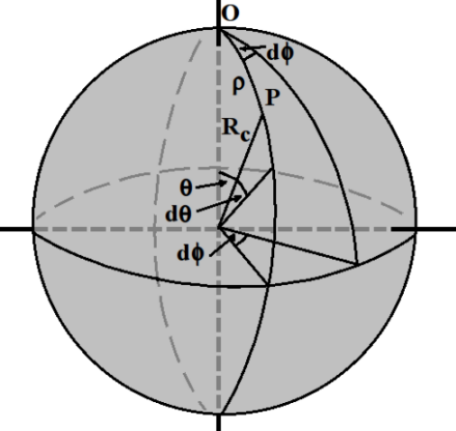
\includegraphics[width=0.5\textwidth]
	{./figures/2_theoretical_framework/2D_Sphere.png}
	
	\caption{\small{Métrica de una superficie esférica.}}
	
	\label{fig:2sphere}
\end{figure}
%.........................................................................



Un elemento de línea sobre la superficie de la figura \ref{fig:2sphere} 
puede ser descrito como


%.........................................................................
%Line element on the sphere
\[ dl^2 = d\rho^2 + R_c^2 \sin^2 \pr{ \frac{\rho}{R_c}}d\phi^2 \]
%.........................................................................
donde se ha introducido una nueva coordenada de longitud sobre la superficie
definida como $\rho = \theta R_c$ y $R_c$ radio de curvatura de la esfera. 
Otra forma muy conveniente de reescribir esta expresión y que permite una
generalización muy útil se logra introduciendo el parámetro de curvatura $k$ 
y la coordenada $r = \sin (\rho/a)$, obteniendo


%.........................................................................
%Line element on the sphere with time-dependent curvature
\[ dl^2 = a^2(t) \cor { \frac{dr^2}{1-kr^2} + r^2 d\phi^2 } \]
%.........................................................................
con $k = -1$ y se asume un radio de curvatura dependiente del tiempo 
$R_c = a(t)$.
La métrica para el caso de 3 dimensiones se obtiene reemplazando el 
diferencial del ángulo $d\phi^2$ por uno de ángulo sólido $d\Omega^2 = 
d\theta^2 + \sin^2\theta d\phi^2$

 
%.........................................................................
%Line element on the 3-sphere
\eq{eq:LineElement3D}
{ dl^2 = a^2(t) \cor { \frac{dr^2}{1-kr^2} + r^2 (d\theta^2 + 
\sin^2\theta d\phi^2)} }
%.........................................................................


Finalmente incluyendo el tiempo, el intervalo espacio-temporal para la 
métrica de espacios curvos isotrópicos y homogéneos queda


%.........................................................................
%Interval element on the 3-sphere
\eq{eq:IntervalCurvedSpaces}
{ ds^2 = c^2 dt^2 - a^2(t) \cor { \frac{dr^2}{1-kr^2} + r^2 (d\theta^2 + 
\sin^2\theta d\phi^2)} }
%.........................................................................


La generalización directa de esta expresión consiste en variar los valores
del parámetro de curvatura $k$ para llegar a la métrica de espacios planos 
($k = 0$), esféricos cerrados ($k = -1$) o abiertos ($k = 1$), tal como
es mostrado en \cite{longair2008} o \cite{padmanabhan1995}.

\
%.........................................................................
%Curved Spaces
\begin{figure}[htbp]
	\centering
	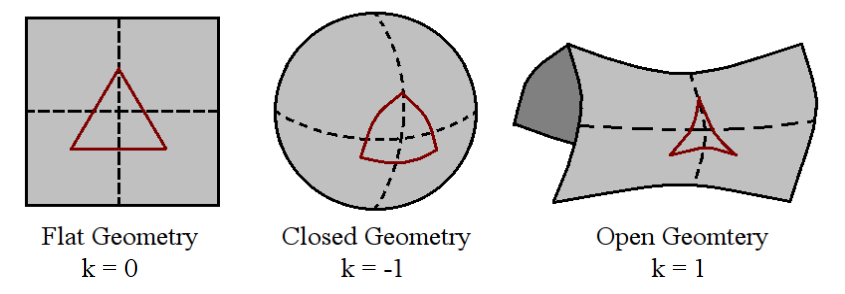
\includegraphics[width=0.9\textwidth]
	{./figures/2_theoretical_framework/Curved_Spaces.png}

	\caption{\small{Diferentes espacios curvos según el parámetro de curvatura.}}
	
	\label{fig:CurvedSpaces}
\end{figure}
%.........................................................................
\

Una manera alternativa de reescribir la métrica es introduciendo dos cambios 
de coordenadas definidos por 


%.........................................................................
%Xi variable
\[ \chi = \int \frac{ dr'}{\sqrt{1 - k r'^2}}\]
%.........................................................................


%.........................................................................
%Proper time
\[ \tau = \int \frac{ c dt'}{a(t')}\]
%.........................................................................
los cuales se interpretan respectivamente como una coordenada de longitud 
sobre la hipersuperficie que define el espacio ($\chi$) y como el tiempo 
propio medido localmente ($\tau$). Se obtiene la siguiente expresiones para 
la métrica


%.........................................................................
%Interval element generalized
\eq{eq:IntervalCurvedSpacesAltern1}
{ ds^2 = c^2 dt^2 - a^2(t) \cor { d\xi^2 +  f^2_k(\xi)(d\theta^2 + 
\sin^2\theta d\phi^2)} }
%.........................................................................


%.........................................................................
%Interval element generalized
\eq{eq:IntervalCurvedSpacesAltern2}
{ ds^2 = \bar a^2 (\tau)\cor{ d\tau^2 - d\xi^2 -  f^2_k(\xi)(d\theta^2 + 
\sin^2\theta d\phi^2)} }
%.........................................................................
donde la función $f_k(\chi)$ es definida de acuerdo al valor del parámetro 
de curvatura


%.........................................................................
%Curvature Function
\eq{eq:CurvatureFunction}
{ f_k(\chi) = \left\{  \matrix{	
\sin \chi	&	k = 1		\cr 
\chi 		& 	k = 0 		\cr	
\sinh \chi 	& 	k = -1 		\cr } \right.  }
%.........................................................................


A pesar de que las expresiones derivadas para la métrica 
\ref{eq:IntervalCurvedSpaces} \ref{eq:IntervalCurvedSpacesAltern1} y
\ref{eq:IntervalCurvedSpacesAltern2} son equivalentes, el uso de una u otra
depende de la conveniencia del problema. En especial la forma 
\ref{eq:IntervalCurvedSpacesAltern1} suele ser más usada y se define como 
métrica de Friedmann.


Puede ser mostrado que en variedades Riemannianas 
\footnote{Una variedad Riemanniana es un espacio donde puede ser definido el 
concepto de métrica.} 
el intervalo espacio-temporal se expresa en términos de la tensor métrico
como \cite{weinberg1972}


%.........................................................................
%Metric-Interval relation
\[ ds^2 = g_{\mu \nu}dx^\mu dx_\nu \]
%.........................................................................
donde se ha introducido el cuadrivector $x^\mu = (ct, r, \theta, \phi)$.


Debido a la asunción de isotropía y homogeneidad el tensor métrico debe ser
diagonal, además comparando con la expresión \ref{eq:IntervalCurvedSpaces}
se llega a la siguiente forma explícita


%.........................................................................
%MetricTensor
\eq{eq:MetricTensor}
{g_{\mu \nu} = \pr{ \matrix{ 
1		&				0			&		0			&				0				\cr
0		&	-a^2(t)(1 - kr^2)^{-1}	&	 	0			&				0				\cr
0		&				0			&	-a^2(t)r^2		&				0				\cr
0		&				0			&		0			&	-a^2(t)r^2 \sin^2 \theta } }}
%.........................................................................


A partir de esta métrica y las ecuaciones de campo de Einstein es posible 
construir sencillos modelos de universo, tal como se muestra a en la 
subsección \ref{subsec:GeneralRelativityAndFriedmannEquations}.


			%-------------------------------------------------------------
			%Medidas de distancias
			\subsubsection*{Medición de distancias}
			%-------------------------------------------------------------
			
Una vez definida la métrica de espacios curvos es útil introducir algunos
conceptos de distancia que son usados de forma recurrente \cite{longair2008}. 
Por simplicidad se asumirá una métrica plana ($k = 0$).

\begin{itemize}
%Comovil Radial Distance..................................................
\item \textit{\textbf{Distancia radial comóvil:}} por definición, una señal 
lumínica tiene asociado un valor nulo del intervalo $ds^2 = 0$, usando la 
métrica \ref{eq:IntervalCurvedSpaces} se llega a


%.........................................................................
%Comovil Distance
\eq{eq:ComovilDistance}
{ r = \int_t^{t_0} \frac{ cdt'}{a(t')} = \int_a ^1 \frac{ c da}{a \dot a} }
%.........................................................................
donde la forma de $a(t)$ depende de la cosmología específica que se use
(ver subsección \ref{subsec:SimpleSolutionsOfTheUniverse}) y $t_0$ es el 
tiempo de referencia, el cual se toma como la edad actual del universo. 


Debido a la asunción de expansión de la métrica, la distancia entre dos 
objetos depende del tiempo en que es medida, y más aún, esta distancia no 
puede ser determinada a partir de un haz de luz debido a la finitud de su
velocidad \footnote{$c=299\ 792\ 458$ m/s}. Por esta razón se debe 
realizar una proyección del cono de luz trazado por el haz en la época 
actual, tal como se hace en la expresión \ref{eq:ComovilDistance}. Esto 
último permite interpretar $r$ como la distancia a un objeto en el tiempo
actual, y es diferente a la distancia aparente que corresponde al 
tiempo en que el objeto emitió la luz que se observa.


%Proper Radial Distance..................................................
\item \textit{\textbf{Distancia radial propia:}} en virtud de la definición
de factor de escala, para obtener la distancia a un objeto en cualquier 
tiempo basta multiplicar su distancia comóvil por el factor de escala en 
ese mismo tiempo, esto es


%.........................................................................
%Proper Distance
\eq{eq:ComovilDistance}
{ r_{\submath{prop}} = a(t)\int_t^{t_0} \frac{ cdt'}{a(t')} = 
a\int_a ^1 \frac{ c da}{a \dot a} }
%.........................................................................	


%Particle Horizon........................................................
\item \textit{\textbf{Horizonte de partículas:}} considerando un haz de 
luz que viaja en el vacío desde el inicio del universo en $t=0$, la máxima 
distancia propia que puede haber recorrido en un tiempo $t$ se denomina 
horizonte de partículas y determina la región que puede estar conectada 
causalmente en el universo en esa época.


%.........................................................................
%Particle Horizon distance
\eq{eq:HorizonDistance}
{ r_{\submath{H}} = a(t)\int_0^{t} \frac{ cdt'}{a(t')} = 
a\int_0 ^a \frac{ c da}{a \dot a} }
%.........................................................................

\end{itemize}
	%---------------------------------------------------------------------
	%General relativity and Friedmann equations
	\subsection{Relatividad General y Ecuaciones de Friedmann}
	\label{subsec:GeneralRelativityAndFriedmannEquations}
	%---------------------------------------------------------------------
	

Las ecuaciones de campo métrico de Einstein desempeñan un papel fundamental
en la relatividad general ya que expresan de forma explícita la relación 
entre la materia y la geometría local del espacio-tiempo.


%.........................................................................
%EinsteinEquations
\eq{eq:EinsteinEquations}
{ R_{\mu \nu} - \frac{1}{2}R - g_{\mu \nu}\Lambda = 
\frac{8\pi G}{c^4}T_{\mu \nu} }
%.........................................................................
o de forma equivalente 


%.........................................................................
%Einstein Equations Alternative
\eq{eq:EinsteinEquationsAltern}
{ R_{\mu \nu} + g_{\mu \nu}\Lambda = 
\frac{8\pi G}{c^4}\pr{T_{\mu \nu} - \frac{1}{2}T g_{\mu \nu}} }
%.........................................................................
donde $T$ es la traza del tensor momentum energía 
(ver \ref{eq:MomentumEnergyTensor}), $R_{\mu \nu}$ el tensor de Ricci y $R
$ el escalar de curvatura. Estos dos últimos calculados a partir de 
trazas del tensor de curvatura de Riemann como 
$R_{\mu \nu} = R^\eta_{\ \mu \eta \nu}$ y $R = R^{\mu}_{\ \mu}$. Por 
conveniencia se ha introducido el término asociado a la constante 
cosmológica y será usado posteriormente para calcular modelos de universo
con energía oscura.


El tensor de Riemann cuantifica la diferencia entre la métrica del espacio-
tiempo curvo y la métrica Euclideana y permite determinar completamente 
las propiedades geométricas como la curvatura local, la medida de
distancias y ángulos, etc \cite{weinberg1972}. Es construido a partir de 
la conexión afín como


%.........................................................................
%Riemann Tensor
\eq{eq:RiemannTensor}
{ R^\mu_{\ \nu \alpha \beta} = 
\Gamma^\mu_{\ \nu \alpha, \beta} -  
\Gamma^\mu_{\ \nu \beta, \alpha} + 
\Gamma^\mu_{\ \sigma \alpha}\Gamma^\sigma_{\ \nu \beta}-
\Gamma^\mu_{\ \sigma \beta}\Gamma^\alpha_{\ \nu \alpha}}
%.........................................................................
a su vez la conexión afín se define en términos de la métrica


%.........................................................................
%Afin Connection
\eq{eq:AfinConnection}
{ \Gamma^\nu _{\ \alpha \beta}  = \frac{1}{2}g^{\mu \sigma}
\pr{ g_{\sigma \alpha, \beta} + g_{\sigma \beta, \alpha} -
g_{\alpha \beta, \sigma} } }
%.........................................................................


El lado derecho de la ecuación \ref{eq:EinsteinEquations} contiene el 
tensor de momentum energía $T_{\mu \nu}$, que caracteriza la densidad y el 
flujo materia-energía en el universo. En virtud del principio cosmológico
este tensor también debe ser diagonal y si además se asume un modelo de 
fluido ideal se obtiene la siguiente forma


%.........................................................................
%MomentumEnergyTensor
\eq{eq:MomentumEnergyTensor}
{T^\mu_{\ \nu} = \pr{ \matrix{ 
c\rho^2	&	0	&	0	&	0				\cr
0		&	-P	&	0	&	0				\cr
0		&	0	&	-P	&	0				\cr
0		&	0	&	0	&	-P } }}
%.........................................................................


Finalmente usando las ecuaciones \ref{eq:MetricTensor}, 
\ref{eq:EinsteinEquationsAltern} y \ref{eq:MomentumEnergyTensor} es posible 
reducir el complejo sistema ecuaciones tensoriales a dos ecuaciones 
escalares acopladas denominadas ecuaciones de Friedmann \cite{longair2008}. 
Estas describen completamente la evolución de un universo isotrópico y 
homogéneo en términos del factor de escala $a(t)$ (ver ecuación
\ref{eq:LineElement3D})


%.........................................................................
%Friedmann Equation 1
\eq{eq:FriedmannEquation1}
{ \frac{\ddot a}{a} = -\frac{4\pi G}{3}\pr{\rho + \frac{3P}{c^2}}
+ \frac{c^2 \Lambda}{3}}
%.........................................................................


%.........................................................................
%Friedmann Equation 2
\eq{eq:FriedmannEquation2}
{ \frac{\ddot a}{a} + 2\frac{\dot a^2}{a^2} + 2\frac{c^2 k}{a^2} =
4\pi G \pr{ \rho - \frac{P}{c^2} } + c^2 \Lambda}
%.........................................................................


Para resolver este sistema en términos de $a(t)$ y obtener así la evolución 
de la escala del universo es necesario conocer la forma en la que cambia la 
densidad $\rho$ y la presión $P$ en el tiempo o el factor de escala, y para 
todos los diferentes tipos de materia-energía del universo. Una derivación 
detallada de estas dependencias puede ser encontrada en \cite{longair2008} y
es resumido en la tabla \ref{tab:PropertiesDependence}

\
%.........................................................................
%Table of dependences of Matter-Energy content of the universe with a
\begin{table}[htbp]
\centering
\begin{tabular}{|c|c|c|c|} \hline
\cellc{\textbf{Propiedad}} 	& 
\cellc{\textbf{Densidad}} 	&
\cellc{ \textbf{Presión}}	& 
\cellc{\textbf{Temperatura}}		\\ \hline

& & &  \\
\textbf{Materia }& $\rho = \rho_0 a^{-3}(t)$ & $p = p_0 a^{-5}(t)$ & $T = T_0 a^{-2}(t)$ \\ 
\small{(bariónica + oscura)} & & &  \\ \hline
& & &  \\
\textbf{Radiación }& $\rho = \rho_0 a^{-4}(t)$ & $p = p_0 a^{-4}(t)$ & $T = T_0 a^{-1}(t)$ \\ 
\small{(+ materia relativista)} & & &  \\ \hline
& & &  \\
\textbf{Vacío }& $\rho = \rho_0 $ & $p = p_0 $ & $-$ \\ 
& & &  \\ \hline
\end{tabular}
\caption{Dependencia de algunas propiedades físicas respecto al factor de escala
\cite{longair2008}.}
\label{tab:PropertiesDependence}
\end{table}
%.........................................................................


Por convención se ha tomado el factor de escala en el presente como
$a_0 = a(t_0) = 1$ y los valores de referencia se definen como
$\rho_0 = \rho(a_0)$, $P_0 = P(a_0)$ y $T_0 = T(a_0)$. Usando las 
ecuaciones de Friedmann, definiendo el parámetro de Hubble 
$H(t) = \dot a/ a$ y la densidad de vacío 
$\rho_\Lambda = c^2\Lambda/8\pi G$ se obtiene


%.........................................................................
%Pre Hubble Equation
\[ \pr{ \frac{\dot a}{a} }^2 = H^2(t) = \frac{ 8\pi G}{3}
\cor{ \rho_{m}\frac{1}{a^{3}} + \rho_{r}\frac{1}{a^{4}} + \rho_{\Lambda} }
- \frac{ c^2 k }{a^2} \]
%.........................................................................


Evaluando esta expresión en el tiempo actual $H(t_0) = H_0$, con $H_0$ la 
constante de Hubble y definiendo la densidad crítica $\rho_c$ como la 
densidad actual necesaria para un universo plano


%.........................................................................
%Critical Density
\eq{eq:CriticalDensity}
{ \rho_c = \frac{3H_0^2}{8\pi G} }
%.........................................................................
se llega a la ecuación de evolución para el parámetro de Hubble


%.........................................................................
%Hubble Equation
\eq{eq:HubbleEquation}
{ H^2(t) = H_0^2 \cor{ 
(1 - \Omega_0)\frac{1}{a^2} +  
\Omega_m \frac{1}{a^3} +
\Omega_r \frac{1}{a^4} +
\Omega_\Lambda} }
%.........................................................................
donde se han introducido los parámetros de densidad $\Omega_i$, definidos 
como la densidad actual de la i-ésima especie en el tiempo actual 
normalizada con la densidad crítica \ref{eq:CriticalDensity}, y 
$\Omega_0 = \sum_i \Omega_i$. Estos parámetros de densidad junto con la 
constante de Hubble hacen parte de los parámetros libres de la teoría y 
deben ser establecidos observacionalmente, lo cual permite caracterizar 
cosmologías particulares. \footnote{\textit{Cosmología} debe ser 
entendida en este contexto como una solución específica de las ecuaciones 
de Friedmann.}


	%---------------------------------------------------------------------
	%Simple solutions of the universe
	\subsection{Soluciones Simples de Universo}
	\label{subsec:SimpleSolutionsOfTheUniverse}
	%---------------------------------------------------------------------


A pesar de que en este punto no ha sido introducido el formalismo de 
pequeñas perturbaciones y la formación de estructuras, el conjunto de 
ecuaciones \ref{eq:FriedmannEquation1}, \ref{eq:FriedmannEquation2} y 
\ref{eq:HubbleEquation} permiten una primera comprensión rudimentaria de 
la evolución del universo.


En esta subsección serán presentadas algunas soluciones analíticas de las 
ecuaciones de Friedmann. A pesar de su carácter ideal, en algunos casos
pueden ser usadas como aproximaciones a algunas etapas de evolución del 
universo, permitiendo así un entendimiento físico más adecuado que 
soluciones numéricas exactas.


			%-------------------------------------------------------------
			%Einstein-de Sitter Universe
			\subsubsection*{Universo Einstein - de Sitter}
			%-------------------------------------------------------------


El universo Einstein-de Sitter es un modelo cosmológico con una métrica 
plana y compuesto enteramente de materia, esto implica que 
$\Omega_0 = \Omega_m = 1$ y $k=0$. Aplicando esto en la ecuación 
\ref{eq:HubbleEquation} se obtiene


%.........................................................................
%EinsteindeSitter
\eq{eq:EinsteindeSitter}
{ H^2(t) = \pr{\frac{\dot a}{a}}^2 = H_0^2 \frac{1}{a^3} }
%.........................................................................


Integrando se llega a la solución para el factor de escala en función del 
tiempo


%.........................................................................
%EinsteindeSitterSolution
\eq{eq:EinsteindeSitterSolution}
{ t(a) = \frac{ 2}{3H_0} a ^{3/2} }
%.........................................................................


A pesar de que en este caso es posible obtener la forma explícita de $a(t)$,
la mayoría de veces solo se tiene una solución implícita de la forma $t(a)$.
Otra forma muy útil de escribir esta solución es en términos del corrimiento
al rojo $z$, el cual se relaciona con el factor de escala como 
\cite{longair2008}


%.........................................................................
%Redshift
\eq{eq:Redshift}
{ z + 1 = \frac{ a_0}{a} }
%.........................................................................
para obtener finalmente


%.........................................................................
%EinsteindeSitterSolutionZ
\eq{eq:EinsteindeSitterSolutionZ}
{ t(a) = \frac{ 2}{3H_0} (1+z) ^{-3/2} }
%.........................................................................


Esta solución se aproxima al comportamiento del universo real en la época
de dominio de la materia, entre $70000$ y $5$ millones de años después del 
Big Bang \cite{padmanabhan1995}.


			%-------------------------------------------------------------
			%Radiation Dominated Universe
			\subsubsection*{Universo dominado por radiación}
			%-------------------------------------------------------------

En este caso se asume un universo dominado completamente por radiación tal
que $\Omega_0 = \Omega_r$, pero no necesariamente plano. La ecuaciones de 
Friedmann conducen entonces a la siguiente expresión


%.........................................................................
%Radiation Universe
\eq{eq:RadiationUniverse}
{ H^2(t) = \pr{\frac{\dot a}{a}}^2 = H_0^2 \cor{ 
(1 - \Omega_r)\frac{1}{a^2} +  \Omega_r \frac{1}{a^4}} }
%.........................................................................


Integrando se obtiene la siguiente solución implícita para el factor de 
escala


%.........................................................................
%Radiation Universe Solution
\eq{eq:RadiationUniverseSolution}
{ t = \left\{  \matrix{ 
H_0^{-1}(\Omega_r - 1)^{-1}\pr{ \Omega_r^{1/2} - 
\cor{a^2(1-\Omega_r) + \Omega_r}^{1/2} } & \Omega_r \neq 1 \cr
H_0^{-1} a^2/2 & \Omega_r = 1} \right. }
%.........................................................................
o en términos del corrimiento al rojo


%.........................................................................
%Radiation Universe Solution Z
\eq{eq:RadiationUniverseSolutionZ}
{ t = \left\{  \matrix{ 
H_0^{-1}(\Omega_r - 1)^{-1}\pr{ \Omega_r^{1/2} - 
\cor{(1+z)^{-2}(1-\Omega_r) + \Omega_r}^{1/2} } & \Omega_r \neq 1 \cr
H_0^{-1} (1+z)^{-2}/2 & \Omega_r = 1} \right. }
%.........................................................................


Esta solución es útil como una aproximación a la época dominada por 
radiación, la cual sucedió desde la creación del universo hasta la 
recombinación, aproximadamente $380 000$ años después del big bang, o 
equivalentemente en un corrimiento al rojo de $z = 1100$ 
\cite{padmanabhan1995}.


			%-------------------------------------------------------------
			%Vacuum Dominated Universe
			\subsubsection*{Universo dominado por vacío}
			%-------------------------------------------------------------
			
Este tipo de universo hipotético corresponde a uno donde solo existe 
energía asociada por vacío, o equivalentemente dominado por la constante 
cosmológica. Haciendo $\Omega_0 = \Omega_\Lambda$ en las ecuaciones de 
Friedmann se llega a 


%.........................................................................
%Vacuum Universe
\eq{eq:VacuumUniverse}
{ H^2(t) = \pr{\frac{\dot a}{a}}^2 = H_0^2 \cor{ 
(1 - \Omega_\Lambda)\frac{1}{a^2} +  \Omega_\Lambda} }
%.........................................................................


Solucionando para $t(a)$


%.........................................................................
%Vacuum Universe Solution
\eq{eq:VacuumUniverseSolution}
{ t = \frac{1}{H_0^2 \Omega_\Lambda^{1/2}}
\ln\cor{ a \pr{ \frac{\Omega_\Lambda}{1 - \Omega_\Lambda} }^{1/2} +
\pr{ 1 + \frac{\Omega_\Lambda}{1 - \Omega_\Lambda}a^2 }^{1/2} } }
%.........................................................................
y respecto al corrimiento al rojo


%.........................................................................
%Vacuum Universe Solution Z
\eq{eq:VacuumUniverseSolutionZ}
{ t = \frac{1}{H_0^2 \Omega_\Lambda^{1/2}}
\ln\cor{ \frac{1}{1+z} \pr{ \frac{\Omega_\Lambda}{1 - \Omega_\Lambda} }^{1/2} +
\pr{ 1 + \frac{\Omega_\Lambda}{1 - \Omega_\Lambda}\frac{1}{\pr{1+z}}^2 }^{1/2} } }
%.........................................................................


Lo interesante de esta solución es que solo es válida para valores del
parámetro de densidad que satisfacen $0<\Omega_\Lambda <1$. Esto muestra 
que no es posible tener universos con geometría plana o hiperbólica cuando 
solo se tiene constante cosmológica. Otro aspecto igual de notable es la 
concavidad de la función $a(t)$ obtenida de \ref{eq:VacuumUniverseSolution}
(ver figura \ref{fig:Cosmologies}), lo que muestra una expansión acelerada
del universo. Esta característica solo es posible cuando hay un término no 
nulo de energía de vacío.


Finalmente y al igual que las anteriores soluciones, la expresión 
\ref{eq:VacuumUniverseSolution} puede ser usada como aproximación a la era
de dominio de vacío del universo, la cual va desde el fin de la era de 
dominio de materia, $5$ millones de años después del 
Big Bang, hasta la actualidad \cite{longair2008}.


			%-------------------------------------------------------------
			%WMAP7 Universe
			\subsubsection*{Universo WMAP7}
			%-------------------------------------------------------------
			
El conjunto de parámetros derivados del modelo cosmológico estándar han 
sido medidos en varias ocasiones por diferentes sondas espaciales (ver 
sección \ref{sec:CosmologicalObservations}), entre estas destaca el WMAP. 
Los datos derivados después de siete años de esta sonda (WMAP7) son los 
adoptados en este trabajo \cite{WMAP7}. Entre los parámetros cosmológicos 
medidos se encuentra la constante de Hubble y los parámetros de densidad 
$\Omega_i$. Tomando los valores de la tabla \ref{tab:CosmologicalParameters} 
y por simplicidad asumiendo $\Omega_0 = 1$ es posible integrar las 
ecuaciones de Friedmann


%.........................................................................
%WMAP Universe
\eq{eq:WMAPUniverse}
{ H^2(t) = H_0^2 \cor{ 
\Omega_m \frac{1}{a^3} +
\Omega_r \frac{1}{a^4} +
\Omega_\Lambda} }
%.........................................................................
para llegar a


%.........................................................................
%WMAP Universe
\eq{eq:WMAPUniverse}
{ t = \frac{1}{H_0}\int _0 ^{a}\cor{ 
\Omega_m \frac{1}{a'} + 
\Omega_r \frac{1}{a'^2} +
\Omega_\Lambda a'^2 }^{-1/2}da' }
%.........................................................................

\
%.........................................................................
%Friedmann Solutions
\begin{figure}[htbp]
	\centering
	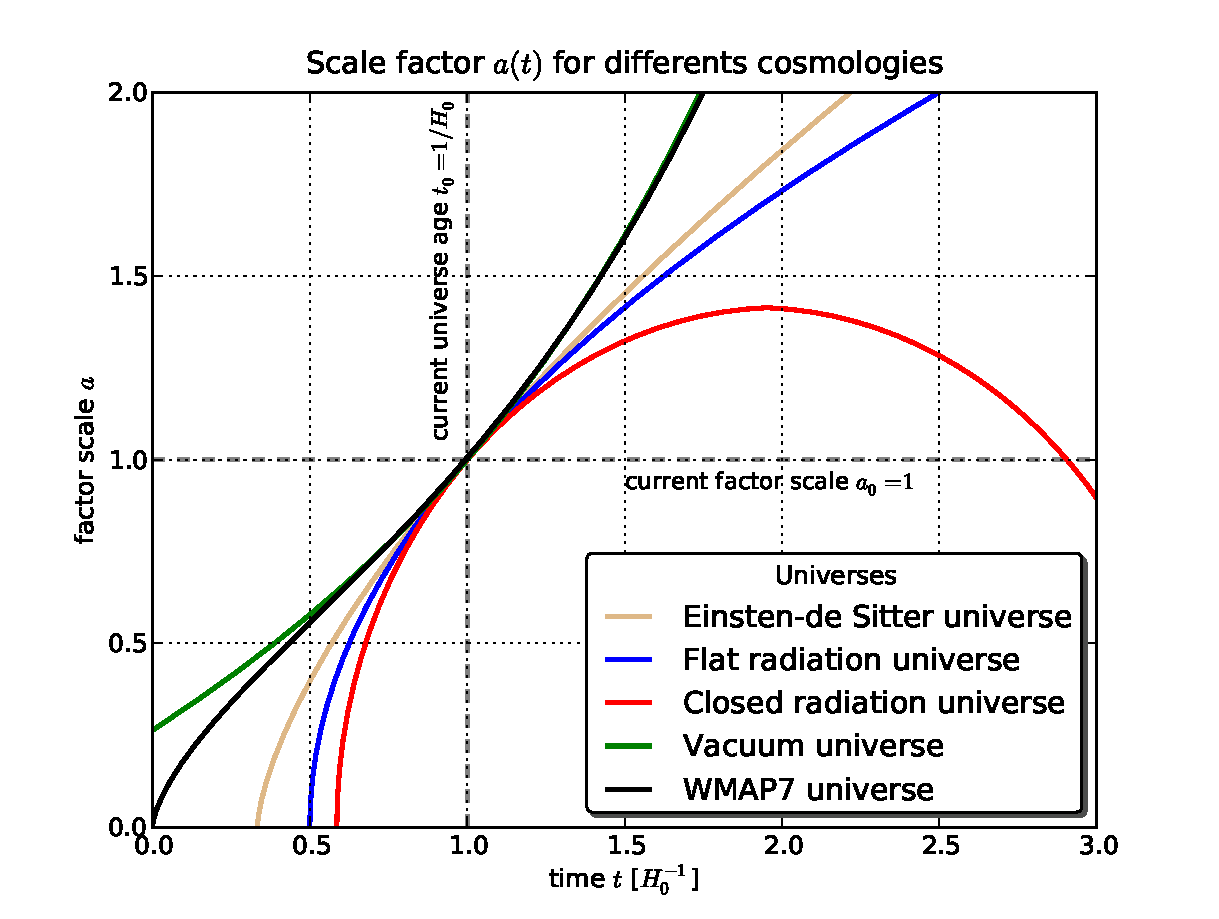
\includegraphics[width=0.9\textwidth]
	{./figures/2_theoretical_framework/Friedmann_Solution.pdf}

	\caption{\small{Diferentes soluciones de universo para las ecuaciones
	de Friedmann.}}
	
	\label{fig:Cosmologies}
\end{figure}
%.........................................................................
\

Es posible obtener una solución analítica de esta integral en términos de 
funciones elípticas, pero por simplicidad se opta por realizar una 
integración numérica. En la figura \ref{fig:Cosmologies} se muestra la 
solución para el universo WMAP7 y se compara con las demás cosmologías 
derivadas previamente.


Una característica interesante de la solución para un universo WMAP7 es
el cambio de concavidad (ver curva negra en la figura \ref{fig:Cosmologies})
que indica que se pasa de un régimen dominado por materia/radiación a uno 
dominado por la expansión acelerada asociada a la energía del vacío. 
Otro aspecto importante es la predicción de la edad el universo. Teniendo 
en cuenta la normalización definida anteriormente para el factor de escala 
$a(t_0) = a_0$, es directo ver que $t_0 = H_0^{-1} \approx 13.75 \times 10^9$ 
años. Otras cosmologías bajo la misma normalización predicen edades
diferentes, desde mayores como el caso del universo de vacío, hasta mucho 
menores e inclusive un tiempo final (big crunch) como el universo con 
geometría cerrada con radiación.


%*************************************************************************




%*************************************************************************
%Linear Structure Formation
\section{Régimen Lineal de Formación de Estructuras}
\label{sec:LinearStructureFormation}


La sección pasada aborda el universo de manera completamente global, 
asumiendo válidas las condiciones de isotropía y homogeneidad. El 
universo real a pesar de tener ese comportamiento de manera asintótica en
escalas muy grandes, en escalas menores es muy diferente, siendo 
completamente anisotrópico y altamente no homogéneo. Un ejemplo claro de 
esto último es la vida, una de las más altas no linealidades del universo,
pasando luego por planetas, estrellas, galaxias, cúmulos galácticos, en 
orden de inhomogeneidad e anisotropía respectivamente.


La forma estándar de introducir estos efectos de estructura en el universo
es asumir válidas las soluciones de Friedmann a grandes escalas y considerar
las inhomogeneidades como perturbaciones del modelo. Pasando primero por el
régimen lineal para el cual las perturbaciones en el campo de densidad son 
mucho menores que el valor medio de fondo ($\delta \rho \ll \rho_b$), hasta 
el régimen no lineal en que son comparables o mayores 
($\delta \rho \sim \rho_b$) sección \ref{sec:NonLinearStructureFormation}).


	%---------------------------------------------------------------------
	%Newtonian Approximation
	\subsection{Aproximación Newtoniana}
	\label{subsec:Newtonian Approximation}
	%---------------------------------------------------------------------


El marco de la evolución lineal puede ser abordado de dos formas. La primera
es considerar un término perturbativo en el tensor momentum-energía 
$ \delta T_{\mu \nu}$ y linealizar las ecuaciones de campo métrico 
\ref{eq:EinsteinEquations} y resolver finalmente para $\delta R_{\mu \nu}$


%.........................................................................
%Perturbative Einstein Equations
\eq{eq:PerturbativeEinsteinEquations}
{ \mathcal{L}( R_{\mu \nu}, \delta R_{\mu \nu} ) = 
\frac{8\pi G}{c^2}\pr{ T_{\mu \nu} + \delta T_{\mu \nu} } }
%.........................................................................


A pesar de que este método es rigurosamente más adecuado, tiene un 
incoveniente que lo hace considerablemente complicado de aplicar, los 
términos perturbativos no lo son necesariamente en todos los sistemas 
coordenados e incluso pueden llegar a ser del mismo orden o mayores que el 
término de fondo \cite{padmanabhan1995}.


El segundo método consiste en asumir perturbaciones con una dimensión 
comóvil menor al radio de Hubble ($r_\delta \ll r_H \sim cH_0^{-1}$) 
\footnote{Un radio de Hubble $r_H$ es una unidad de longitud que define 
el orden de magnitud del tamaño del universo observable.}, y así 
despreciar los efectos relativistas debido a la curvatura de la 
espacio-tiempo. Una vez hecho esto es posible usar un esquema Newtoniano 
para el desarrollo de las perturbaciones en el universo de fondo, este 
esquema asume el contenido de materia como un fluido y está soportado por 
tres ecuaciones básicas de la mecánica de fluidos. La primera es la 
ecuación de continuidad que representa la conservación de la masa del 
fluido


%.........................................................................
%Continuity equation
\eq{eq:ContinuityEquation}
{ \dtot{\rho}{t} = - \rho \nabla \cdot \bds u }
%.........................................................................


La segunda es la ecuación de Euler que caracteriza el campo de velocidades
del fluido y físicamente representa la conservación del momentum


%.........................................................................
%Euler Equation
\eq{eq:EulerEquation}
{ \dtot{\bds u}{t} = -\frac{ \nabla P}{\rho} - \nabla \varphi }
%.........................................................................


Y finalmente la ecuación de Poisson que es la forma no relativista de las 
ecuaciones de campo de Einstein y especifica el contenido de materia como
fuentes de campo gravitacional.
	
	
%.........................................................................	
%Poisson Equation
\eq{eq:PoissonEquation}
{ \nabla^2 \varphi = 4\pi G \rho }
%.........................................................................	


Para completar el marco Newtoniano de perturbaciones es necesario incluir 
en el anterior sistema de ecuaciones (\ref{eq:ContinuityEquation}, 
\ref{eq:EulerEquation} y \ref{eq:PoissonEquation}) el efecto de la 
expansión del universo, para esto se realiza un cambio de coordenadas de
distancia propia $\bds x$ a distancia comóvil $\bds r$


%.........................................................................	
%Changing Coordinate
\[\bds x = a \bds r\]
%.........................................................................	
esto implica directamente que


%.........................................................................	
%Changing Coordinate
\[\bds u = \dtot{\bds x}{t} = 
\frac{\dot a}{a}\bds x + \bds v = \dot a \bds r + \bds v\]
%.........................................................................	


Esta forma de reescribir $\bds u$ permite separar la componente debida a la
expansión del universo ($\dot a/a \bds x$), o también denominada Ley de 
Hubble, de la componente debida al movimiento del fluido, denominado campo 
de velocidad peculiar y es definido como $\bds v = a \dot{ \bds r}$.

	
Por conveniencia se descompone el campo de densidad del fluido en una parte 
media o de fondo y en una parte perturbativa, esto es 
$\rho = \bar \rho + \delta\rho = \bar \rho( 1+ \delta )$, donde $\delta$ se 
denomina parámetro de densidad y es adimensional. En el caso del potencial 
gravitacional $\varphi$ se define un nuevo campo dado por 
$ \Phi = \phi + \ddot a a r^2/2$ \cite{longair2008}. Con estas 
consideraciones se obtiene finalmente el conjunto final de ecuaciones
de fluido para el marco Newtoninano


%.........................................................................	
%Fluid Equations
\begin{eqnarray}
%.........................................................................	
\label{eq:ContinuityEquationC}
\matrix{\mbox{\footnotesize{Ecuación de}} \cr \mbox{\footnotesize{continuidad}}} & &
\der{\delta}{t} = - \frac{1}{a}\nabla_r \cdot \cor{ (1+\delta)\bds v }\\
\nonumber{}
\\
%.........................................................................	
\label{eq:EulerEquationC}
\matrix{\mbox{\footnotesize{Ecuación de}} \cr \mbox{\footnotesize{Euler}}} & &
\der{\bds v}{t} + \frac{\dot a}{a}\bds v + 
\frac{1}{a}\pr{ \bds v\cdot \nabla_r }\bds v = 
-\frac{\nabla_r P}{a \bar \rho(1+\delta)} - 
\frac{1}{a}\nabla_r \Phi \\
\nonumber{}
\\
%.........................................................................	
\label{eq:PoissonEquationC}
\matrix{\mbox{\footnotesize{Ecuación de}} \cr \mbox{\footnotesize{Poisson}}} & &
\nabla^2_r \Phi = 4\pi G\bar \rho a^2 \delta
\end{eqnarray}
%.........................................................................	


Hasta este punto no se ha hecho explícito el tipo de contenido 
materia-energía que es perturbado con las ecuaciones de fluido (e.g. 
radiación, materia o energía oscura). Siguiendo el procedimiento para 
derivar el anterior sistema puede notarse que no se ha hecho ninguna 
suposición a priori sobre comportamiento de las variables de estado respecto
al factor de escala (ver tabla \ref{tab:PropertiesDependence}), por tanto 
son válidas para cualquiera de las especies
\footnote{De acá en adelante cada uno de los tipos de materia-energía que 
contribuyen al tensor momentum-energía serán denominados \textit{especies}.} 
presentes en el universo. Teniendo en cuenta que las estructuras del universo 
actual son completamente de materia, solo se usará el marco Newtoniano para 
perturbaciones de esta especie.


Las cantidades físicas que deben ser determinadas a partir de las ecuaciones
de fluido, sumadas a las ecuaciones de Friedmann son: el parámetro de 
densidad $\delta$, el campo de velocidad peculiar $\bds v$, el potencial
efectivo $\Phi$, la presión $P$ y finamente el factor de escala $a$. Es 
claro entonces que debe incluirse una ecuación extra para la completa
autoconsistencia del problema, esto se logra a partir de una ecuación de 
estado para la presión. Por simplicidad se asume un modelo de gas 
monoatómico de la materia para el cual la ecuación estado satisface


%.........................................................................	
%EOS equation
\eq{eq:EOSEquation}
{ \nabla_r P = c_s^2 \bar \rho \nabla \delta + 
\frac{2}{3}\bar T \rho \nabla s }
%.........................................................................	
donde $c_s$ es la velocidad del sonido en el medio, $\overline T$ la 
temperatura de fondo y $s$ la entropía específica. Usando esta expresión 
junto con \ref{eq:ContinuityEquationC} y \ref{eq:EulerEquationC} se llega
a la ecuación general para la evolución de las perturbaciones


%.........................................................................	
%Delta Evolution
\eq{eq:DeltaEvolution}
{ \der{^2 \delta}{t^2} + 2\frac{\dot a}{a} \der{\delta}{t} = 
4\pi G \bar \rho \delta + \frac{c_s^2}{2}\nabla^2 \delta +
\frac{2}{3}\frac{\overline T}{a^2}\nabla^2 s }
%.........................................................................	


En el régimen lineal $\delta \ll 1$ los modos del campo de densidad 
evolucionan de forma independiente, permitiendo así desacoplar las
perturbaciones de diferentes escalas de tamaño. Una forma bastante estándar 
de resolver este tipo de problemas es usando transformaciones de Fourier, 
esto debido a que en el espacio recíproco los modos son naturalmente 
desacoplados.


Puesto que se han asumido perturbaciones menores al radio de Hubble, el
el volumen de universo observable puede considerarse finito, y por tanto 
la descomposición de los campos en coordenadas comóviles se hace discreta, 
obteniendo


%.........................................................................	
%Fourier Descomposition of Fields
\[  \delta(\bds r, t) =  \sum_{\bds k}\delta_{\bds k} e^{i \bds k \cdot \bds x} 
\ \ \ \ \ 
	\bds v(\bds r, t) =  \sum_{\bds k}\bds v_{\bds k} e^{i \bds k \cdot \bds x}\]
\eq{eq:FourierFields}
{  s(\bds r, t) =  \sum_{\bds k}s_{\bds k} e^{i \bds k \cdot \bds x} 
\ \ \ \ \ 
	\Phi(\bds r, t) =  \sum_{\bds k}\Phi_{\bds k} e^{i \bds k \cdot \bds x}}
%.........................................................................	


Si se asumen perturbaciones adiabáticas, es decir, perturbaciones que no 
intercambian calor con el entorno (universo de fondo) mientras evolucionan,
la entropía específica debe permanecer homogénea y por tanto $\nabla_r s = 0$
\cite{longair2008}. Teniendo esto en cuenta y usando las anteriores 
descomposiciones de los campos se llega al siguiente conjunto de ecuaciones
para la evolución de los modos de densidad y de velocidad peculiar de las 
perturbaciones


%.........................................................................	
%Modes Evolution Equation
\begin{eqnarray}
%.........................................................................	
\label{eq:ContinuityEquationCMode}
\dtot{^2 \delta_{\bds k}}{t^2} + 2\frac{\dot a}{a}\dtot{\delta_{\bds k}}{t} &=& 
\cor{ 4\pi G \bar \rho - \frac{c_s^2}{a^2}k^2 }\delta_{\bds k}\\
\nonumber{}
\\
%.........................................................................	
\label{eq:EulerEquationCMode}
- k^2 \Phi_{\bds k} &=& 4\pi G \bar \rho a^2 \delta_{\bds k}\\
\nonumber{}
\\
%.........................................................................	
\label{eq:PoissonEquationCMode}
\bds v_{\bds k} &=& \frac{i a \bds k}{k^2}\dtot{\delta_{\bds k}}{t}
\end{eqnarray}
%.........................................................................	


	%---------------------------------------------------------------------
	%Jeans Instability
	\subsection{Inestabilidad de Jeans}
	\label{subsec:JeansInstability}
	%---------------------------------------------------------------------
	
	
Las soluciones de la ecuación \ref{eq:ContinuityEquationCMode} para los 
modos del campo de densidad pueden ser clasificadas en dos familias, la 
primera son soluciones donde la amplitud de los modos oscilan en el tiempo
y no colapsan. La segunda familia son aquellas donde los modos crecen en el 
tiempo, colapsando y volviéndose altamente no lineales ($\delta_k \gg 1$). 
Un ejemplo sencillo que ilustra lo anterior y puede ser generalizado 
consiste en considerar perturbaciones en un universo estático, es decir 
$\dot a = 0$. Teniendo en cuenta esto la ecuación 
\ref{eq:ContinuityEquationCMode} toma la forma


%.........................................................................	
%JeansEquation
\eq{eq:JeansEquation}
{\dtot{^2 \delta_{\bds k}}{t^2} -\omega_k^2 \delta_{\bds k} = 0,\ \ \ a=\mbox{cte}}
%.........................................................................	
donde se ha definido la frecuencia característica $\omega_k$ como


%.........................................................................	
%JeansFrequency
\eq{eq:JeansFrequency}
{\omega_k^2 = \cor{\frac{c_s^2}{a^2}k^2 -  4\pi G \bar \rho} }
%.........................................................................	
	

La expresión \ref{eq:JeansEquation} es denominada ecuación de Jeans y 
tiene la forma de una ecuación de ondas, con base en esto las soluciones 
pueden ser clasificadas según el valor de $\omega_k$, tal como se había
mencionado inicialmente.


%.........................................................................	
%Jeans Criteria
\begin{itemize}
\item Si $\omega_k^2>0$ el modo $\delta_{\bds k}$ se comporta de forma 
oscilatoria, manteniendo su amplitud constante en el tiempo. Esta solución
no es de interés para el contexto de formación de estructuras debido a que
no es posible llegar tener colapso gravitacional.

\item Si $\omega_k^2<0$ la amplitud del modo $\delta_{\bds k}$ crece en el 
tiempo, permitiendo el colapso y la formación de estructuras no lineales.
\end{itemize}
%.........................................................................	


La expresión \ref{eq:JeansFrequency} para $\omega_k$ junto con el anterior 
criterio para determinar el tipo de solución permite definir la longitud 
de Jeans $\lambda_J$


%.........................................................................	
%JeansLength
\eq{eq:JeansLength}
{ \lambda_J = \frac{ 2\pi a^2}{k_J} = 
c_s \pr{ \frac{\pi}{G \bar \rho} }^{1/2} }
%.........................................................................	


Esta longitud se interpreta como el mínimo tamaño en coordenadas comóviles 
que debe tener una perturbación embebida en un medio homogéneo y estático
de densidad $\bar \rho$ para colapsar gravitacionalmente. En este mismo 
contexto es posible definir la masa de Jeans como la mínima masa necesaria
para el colapso.


%.........................................................................	
%JeansMass
\eq{eq:JeansMass}
{ M_J = \frac{4}{3}\pi \lambda_J^3 \propto \frac{c_s^3}{G^{3/2}\bar \rho ^{1/2}} }
%.........................................................................


A pesar de que lo derivado anteriormente solo es estrictamente válido para 
medios estáticos, la importancia de su consideración es debida a dos 
razones: la primera es el interés histórico, ya que el problema de 
perturbaciones que crecen en medios homogéneos surge inicialmente en 
astronomía estelar, donde es necesario calcular la masa mínima de una 
perturbación para su colapso y posterior formación de estrellas y sistemas 
planetarios. La segunda razón de debe a que la solución para medios 
estáticos sirve para evaluar el comportamiento asintótico y la validación 
de las soluciones generales para medios en expansión.


Antes de proseguir con las soluciones para medios en expansión es 
conveniente usar las definiciones de longitud y masa de Jeans como 
aproximaciones al caso general, para esto se usa la tabla de propiedades en
función del factor de escala \ref{tab:PropertiesDependence} y la definición 
de la velocidad del sonido en un medio \cite{pathria1996}
	

%.........................................................................	
%SoundVelocity
\eq{eq:SoundVelocity}
{ c_s^2 = \pr{ \der{P}{\rho} }_s }
%.........................................................................


%.........................................................................
%Jeans length and mass
\begin{itemize}
%Matter perturbations
\item En el caso de perturbaciones de materia bariónica se usa la ecuación 
de estado de gas ideal asumiendo hidrógeno atómico y se obtiene la
siguiente expresión para la masa de Jeans


%.........................................................................	
%MatterJeansMass
\eq{eq:MatterJeansMass}
{ M_{J} \approx 9.97\times 10^5
\pr{ \frac{a_{\submath{rc}}}{a} }^{3/2} \mbox{ M}_{\odot}}
%.........................................................................


Por conveniencia se ha introducido el factor de escala correspondiente a la 
época de recombinación \footnote{Época en la que se desacopla la
materia y la radiación, sucede en un corrimiento al rojo aproximadamente de
$z_{\submath{rc}}\approx 1000$.}$a_{\submath{rc}}$.


%Radiation perturbations
\item Para perturbaciones de radiación y materia relativista se usa la 
ecuación de estado de la presión de radiación del campo electromagnético 
\cite{jackson1999} $P = c^2\rho/3$ y la ley de Stefan-Boltzmann
$\rho \propto T^4$, se obtiene la siguiente masa de Jeans


%.........................................................................	
%RadiationJeansMass
\eq{eq:RadiationJeansMass}
{ M_{J} \approx 8.39 \times 10 ^{27} a^3 \mbox{ M}_{\odot}}
%.........................................................................
\end{itemize}
%.........................................................................

	
Ambos casos pueden ser usados como aproximaciones a diferentes estadios del 
universo. Antes de la época de recombinación, cuando la materia y la 
radiación estaban acopladas vía efecto Compton, las perturbaciones solo 
colapsan si tienen una masa aproximada a la masa de Jeans 
\ref{eq:RadiationJeansMass}. Después de esta época, cuando la materia 
evoluciona de forma independiente es válida la expresión 
\ref{eq:MatterJeansMass}.


En la figura \ref{fig:JeansMass} se ilustra el cambio de la masa de Jeans
respecto al factor de escala del universo. Es interesante notar que antes 
de la época de recombinación la formación de estructuras poco masivas era
impedida, lo que se debe al proceso de homogeneización producido por la 
difusión de fotones en el medio. Luego de esta época, cuando surgen las 
perturbaciones de materia bariónica, es posible la formación de estructuras 
menos masivas (del orden de cúmulos globulares), lo que está acorde con la
teoría de formación jerárquica de estructuras a gran escala.

	
%.........................................................................
%Jeans Mass Evolution
\begin{figure}[htbp]
	\centering
	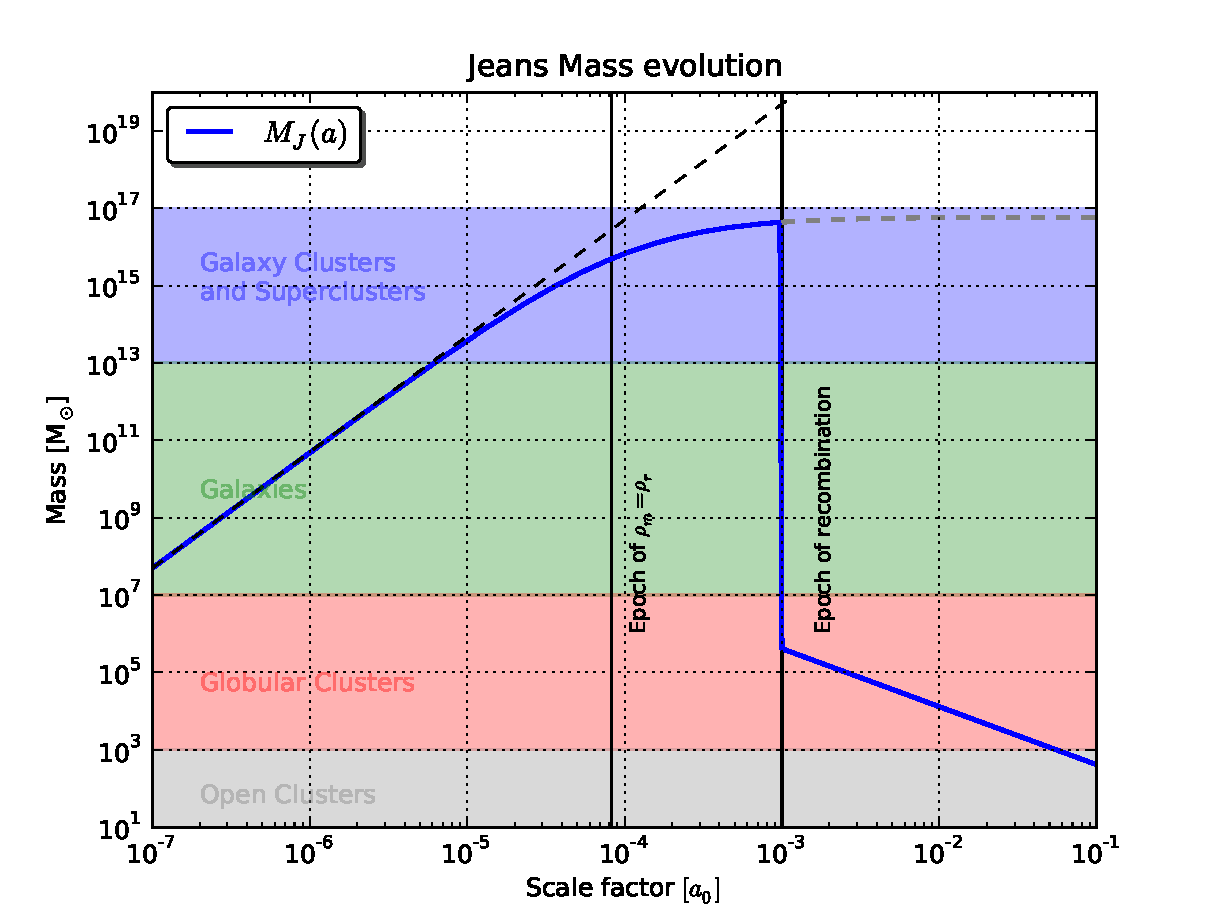
\includegraphics[width=0.9\textwidth]
	{./figures/2_theoretical_framework/Jeans_Mass_Evolution.pdf}

	\caption{\small{Evolución de la masa de Jeans para diferentes estadios
	del universo. En las regiones coloreadas se ilustra el rango típico de 
	masa para varios tipos de estructuras, desde cúmulos estelares abiertos
	hasta cúmulos y supercúmulos de galaxias.}}
	
	\label{fig:JeansMass}
\end{figure}
%.........................................................................	
	

Con el anterior análisis se ha establecido la masa mínima necesaria para 
el colapso de una perturbación, a continuación se estudia la evolución de
tales perturbaciones en medios en expansión. Para esto se hace uso de los
modelos de universo derivados en la subsección 
\ref{subsec:SimpleSolutionsOfTheUniverse} y la ecuación general de evolución
de perturbaciones \ref{eq:ContinuityEquationCMode}.


%.........................................................................
%Solutions to Perturbations Evolution
\begin{itemize}
\item \textbf{Universo Einstein - de Sitter}


Recordando que para este tipo de universo $\Omega_m = \Omega_0 = 1$, usando
la función de Hubble \ref{eq:EinsteindeSitter}, la solución para el factor 
de escala \ref{eq:EinsteindeSitterSolution} y la velocidad del sonido 
derivada de \ref{eq:SoundVelocity} y la ecuación de estado de gas ideal se 
llega a la siguiente expresión para la evolución de las perturbaciones


%.........................................................................	
%Einsten-de Sitter Perturbations
\eq{eq:EinstendeSitterPerturbations}
{ \delta_{\bds k}(a) = \delta_{\bds k, 0} \pr{\frac{a}{a_{\submath{ref}}}}^{1} }
%.........................................................................
donde $\delta_{\bds k, 0}$ son las condiciones del campo en el tiempo de 
referencia $t_{\submath{ref}}$. Otra solución posible es de la forma
$\delta_{\bds k}\propto a^{-3/2}$, pero debido a que es una solución que
decae en el tiempo, no es de interés.


%Radiation Dominated Universe
\item \textbf{Universo dominado por radiación}


Para el caso de perturbaciones en un universo dominado por radiación con
$\Omega_r = \Omega_0 = 1$, usando \ref{eq:RadiationUniverseSolution} se 
llega a


%.........................................................................	
%Radiation Perturbations
\eq{eq:RadiationPerturbations}
{ \delta_{\bds k}(a) = \delta_{\bds k, 0} \pr{\frac{a}{a_{\submath{ref}}}}^{1.22} }
%.........................................................................
donde de nuevo $\delta_{\bds k, 0}$ representa los modos iniciales del 
campo y se ignoran soluciones divergentes.


%Vacuum Dominated Universe
\item \textbf{Universo dominado por vacío}
			

Para un universo de constante cosmológica $\Omega_\Lambda$
\footnote{$\Omega_\Lambda < 1 $ para garantizar convergencia de las soluciones
de la ecuación de Friedmann (ver subsección 
\ref{subsec:SimpleSolutionsOfTheUniverse}).}
se tiene el siguiente comportamiento para la evolución de los modos


%.........................................................................	
%Vacuum Perturbations
\eq{eq:VacuumPerturbations}
{ \delta_{\bds k}(a) = \delta_{\bds k, 0} \pr{\frac{a}{a_{\submath{ref}}}}^{0.58} }
%.........................................................................
\end{itemize}
%.........................................................................


Graficando cada una de estas soluciones se obtiene la figura 
\ref{fig:DeltaEvolution}. Por simplicidad y para ilustrar mejor el 
comportamiento con el factor de escala se normaliza cada solución respecto 
a su valor en el tiempo de referencia $\delta_{\bds k, 0}$. 


Las condiciones iniciales dependen del número de onda comóvil $\bds k$ y
deben ser determinadas a partir de las propiedades estadísticas del campo 
de densidad (ver subsección \ref{subsec:StatisticalProperties}) y de 
medidas observacionales (por ejemplo la radiación cósmica de fondo).

\newpage

%.........................................................................
%Perturbations Evolution
\begin{figure}[htbp]
	\centering
	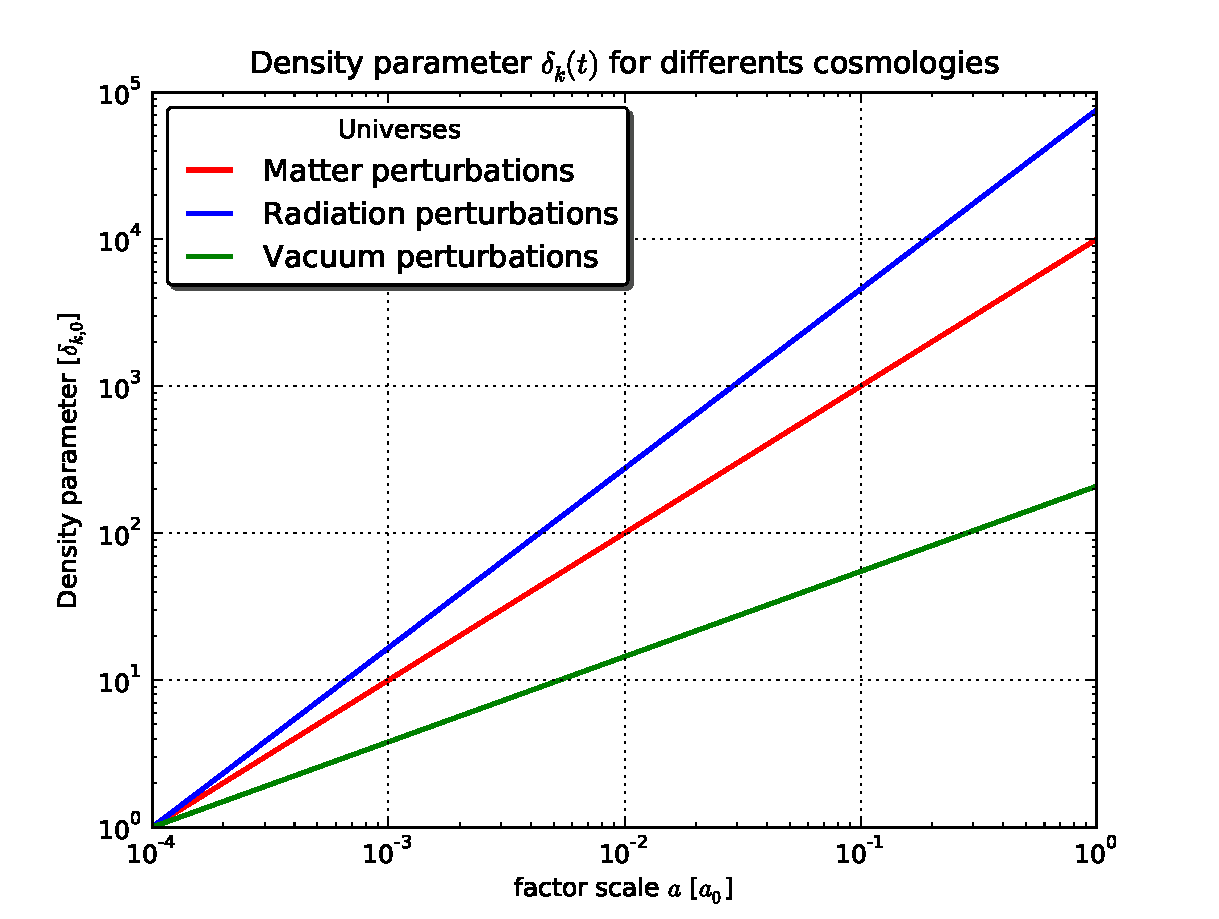
\includegraphics[width=0.9\textwidth]
	{./figures/2_theoretical_framework/Perturbations_Evolution.pdf}

	\caption{\small{Evolución de los modos normales del campo de densidad.
	Por motivos ilustrativos se ha normalizado respecto a las condiciones 
	iniciales.}}
	
	\label{fig:DeltaEvolution}
\end{figure}
%.........................................................................	


	%---------------------------------------------------------------------
	%Statistical Properties and Transfer function
	\subsection{Propiedades Estadísticas y Función de Transferencia}
	\label{subsec:StatisticalProperties}
	%---------------------------------------------------------------------


Una vez determinada la evolución de los modos de densidad es necesario 
compararlos con el universo real. Debido a la naturaleza continua de 
los campos es inviable tratar de determinar de forma ob\-servacional la 
distribución de densidad, más aún, teniendo en cuenta que la mayor parte de 
la materia es oscura, la cual solo puede ser inferida de forma indirecta,
resulta también técnicamente imposible con los instrumentos actuales llevar 
a cabo esta empresa.


A pesar de lo anterior es posible aún medir las propiedades estadísticas
de la distribución de densidad del universo y comparar con lo obtenido de
forma teórica. Para esto se introduce el concepto de funcional de 
probabilidad para un campo continuo $P\cor{ \delta(\bds r,t) }$, definido 
como la probabilidad de que un cierto campo físico tenga la forma funcional 
específica $\delta(\bds r,t)$.


Una manera más conveniente, en términos computacionales, de aplicar el 
formalismo de funcional de probabilidad se logra discretizando el espacio 
en celdas de volumen $\Delta^3 \bds r_i$, de tal forma que una cierta 
forma funcional del campo de densidad $\delta(\bds r,t)$ sea equivalente a 
tener simultáneamente en cada celda $\bds r_i$ del grid el valor 
$\delta_i = \delta(\bds r_i)$, así el funcional de probabilidad se 
transforma en una función de probabilidad conjunta


%.........................................................................
%Probability Functional
\eq{eq:ProbabilityFunctional}
{ P\cor{ \delta(\bds r,t)} \ \ \longrightarrow \ \ 
\mathcal{P}_{\bds{r}}(\delta_1,\delta_2,\cdots,\delta_N;t)  }
%.........................................................................


Teniendo en cuenta la descomposición de Fourier del campo de densidad 
$\delta(\bds r,t)$ en las ecuaciones \ref{eq:FourierFields}, es posible 
definir una función de probabilidad conjunta en el espacio recíproco 
$\mathcal{P}_{\bds k}(\delta_{\bds k_1},\delta_{\bds k_2}, \cdots,
\delta_{\bds k_N};t)$ que caracteriza completamente la probabilidad de 
una distribución específica $\delta_{\bds k}(t)$.


La principal motivación de trabajar en el espacio recíproco de debe a que
es posible usar la aproximación de modos incorrelacionados en la cual se
asume que cada modo evoluciona de forma independiente. En el espacio real 
no es posible realizar esto debido a que el largo alcance de la interacción
gravitacional acopla fuertemente el campo densidad entre diferentes 
lugares. Una consecuencia directa de la anterior aproximación es expresar 
la función de probabilidad conjunta como el producto de $N$ distribuciones
individuales \cite{padmanabhan1995}


%.........................................................................
%Probability Functional Recipro
\eq{eq:ProbabilityJointFour}
{ \mathcal{P}_{\bds k}(\delta_{\bds k_1},\delta_{\bds k_2},
\cdots,\delta_{\bds k_N};t) = \prod_{\bds k_i}g_{\bds k_i}( \delta_{\bds k_i};t )  }
%.........................................................................
donde 


%.........................................................................
%Inverse Fourier Delta
\eq{eq:InverseFourierDelta}
{ \delta_{\bds k} = 
\int_V \delta(\bds r) e^{-i \bds k \cdot \bds r} d^3 \bds r  }
%.........................................................................
$g_{\bds k_i}$ la distribución individual de cada modo, $V=L^3$ el volumen 
de normalización y $\bds k = (2\pi/L)\bds n$, con $\bds n$ un vector de 
componentes enteras que caracterizan el modo específico.


Asumiendo que las perturbaciones primordiales del campo de densidad se 
ori\-ginaron por el proceso de inflación cósmica, es posible demostrar que 
la distribución de los modos normales $g_{\bds k_i}$ es una función 
Gaussiana \cite{padmanabhan1995}. Por conveniencia se descompone en 
coordenadas polares complejas el modo de densidad $\delta_{\bds k} = 
r_{\bds k}\exp\pr{ i \phi_{\bds k} }$, obteniendo la siguiente distribución


%.........................................................................
%Gaussian Distribution
\eq{eq:GaussianDistribution}
{ g_{\bds k}( r_{\bds k}, \phi_{\bds k}; t ) = 
\frac{2(r_{\bds k} dr_{\bds k})}{\sigma_k^2}\pr{ \frac{d\phi_{\bds k}}{2\pi} }
\exp\pr{ -\frac{r_{\bds k}^2}{\sigma_k^2} };\ \ \ \ \ \sigma_k^2 = 2\mu_k^2  }
%.........................................................................
donde $\mu_k^2$ es la varianza de la distribución y $\sigma_k^2$ se 
denomina espectro de potencia. Debido a la asunción de isotropía y 
homogeneidad para el universo de fondo, ambas cantidades solo dependen de 
la magnitud del vector de onda $|\bds k| = k$. También es directo mostrar 
las siguientes propiedades de la distribución del campo


%.........................................................................
%Distribution Properties
\eq{eq:Distribution Properties}
{ \bra \delta_{\bds k} \ket = 0;\ \ \ \ \ 
  \bra |\delta_{\bds k}|^2 \ket = \sigma_k^2;\ \ \ \ \ 
  \bra \delta_{\bds k} \delta_{\bds p}\ket = 0\ \ \ \mbox{si}\ \ \ \
  \bds k \neq \bds p }
%.........................................................................


%.........................................................................
%Initial density
\begin{figure}[htbp]
	\centering
	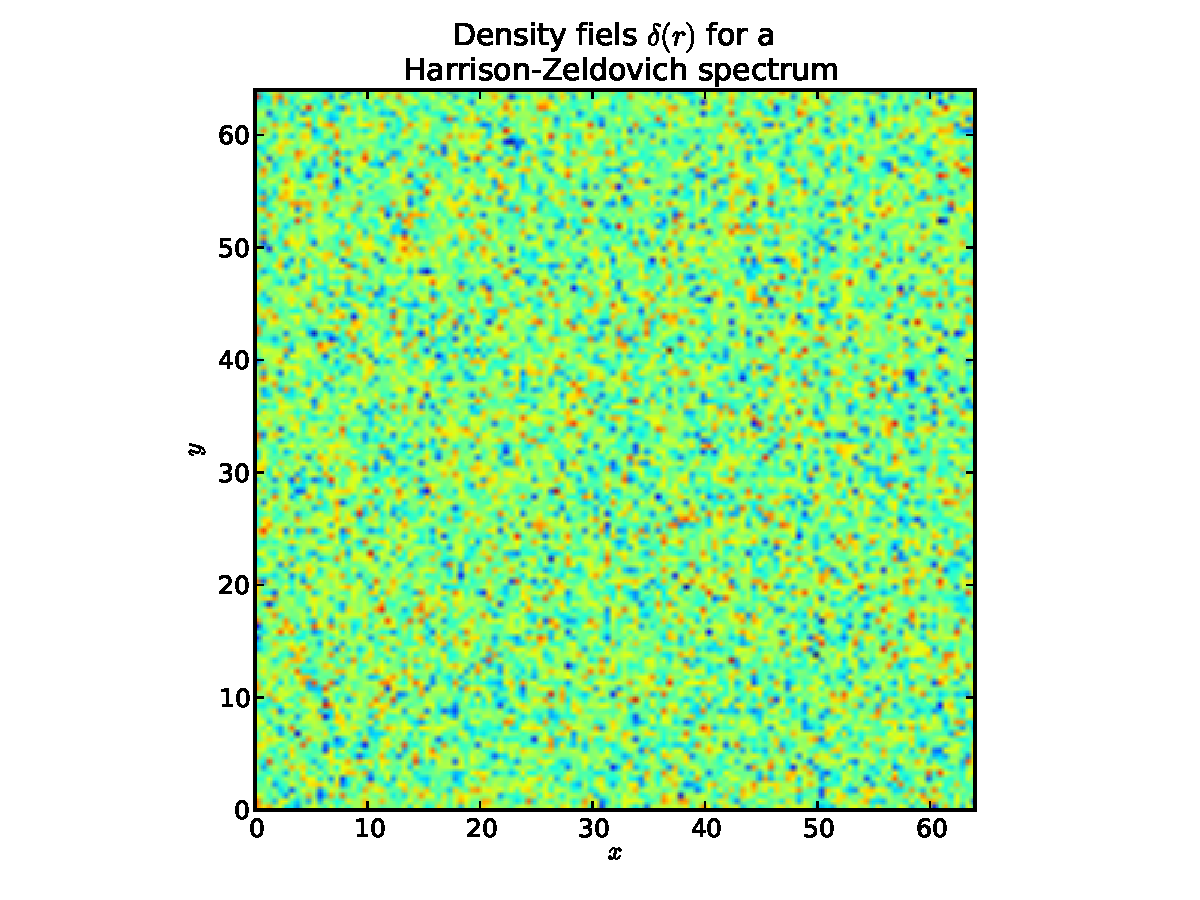
\includegraphics[width=0.9\textwidth]
	{./figures/2_theoretical_framework/Initial_Density.pdf}

	\caption{\small{Distribución inicial de perturbaciones para el campo
	de contraste de densidad a partir de la distribución Gaussiana 
	\ref{eq:GaussianDistribution} y el espectro de potencia de Harrison-
	Zeldovich $\sigma_k \propto k$.}}
	
	\label{fig:InitialDensity}
\end{figure}
%.........................................................................	


Una cantidad que puede ser evaluada directamente es la función de 
correlación de dos puntos $\xi(\bds r) \equiv \bra \delta(\bds r' + \bds r)
\delta(\bds r') \ket$, definida como la probabilidad de tener una 
perturbación a una distancia $\bds r$ de otra. Es una medida directa del 
grado de anisotropía y las propiedades de clustering de una distribución.


%.........................................................................
%Two Points Correlation Function
\begin{eqnarray}
\nonumber
\xi(\bds r) = \bra \delta(\bds r' + \bds r) \delta(\bds r') \ket &=& 
\frac{1}{V^2}\sum_{\bds k, \bds p} \bra \delta_{\bds k} \delta_{\bds p}^*\ket
\exp\cor{ i\bds k \cdot(\bds r' + \bds r)- i\bds p \cdot \bds r' } \\
\label{eq:2PCorrelation}
&=& \int \frac{V^{-1}}{(2\pi)^3}\sigma_k^2 e^{i \bds k \cdot \bds r} d^3 \bds k
\end{eqnarray}
%.........................................................................
donde en la última línea se ha realizado el límite al continuo. La 
expresión \ref{eq:2PCorrelation} muestra que $\sigma_k^2$ es la 
transformada de Fourier de la función de correlación, es decir


%.........................................................................
%Two Points Correlation Function Fourier
\eq{eq:2PCorrelationF}
{ V^{-1}\sigma_k^2 = \int \xi(\bds r) e^{-i\bds k\cdot \bds r}d^3 \bds r }
%.........................................................................


La anterior relación junto con la distribución Gaussiana del campo muestra 
que tanto el espectro de potencia como la función de correlación contienen
toda la información estadística del campo de densidad en el régimen lineal.
En caso de asumir una distribución no-Gaussiana es necesario tener más
momentos de la distribución, tal como la función de correlación de tres 
puntos, etc.


			%-------------------------------------------------------------
			%Harrison-Zeldovich Power Spectrum
			\subsubsection*{Espectro de potencia de Harrison-Zeldovich}
			%-------------------------------------------------------------
			

Una primera aproximación al espectro de potencia, y que puede ser 
demostrada con el modelo de inflación cósmica para las perturbaciones 
primigenias \cite{padmanabhan1995}, es una ley de potencia de la forma


%.........................................................................
%Power Spectrum power
\eq{eq:PowerSpectrumPower}
{ \sigma_k^2 = A k^{n_s} }
%.........................................................................
donde $A$ es un factor de normalización y $n$ es el índice espectral. En 
el caso específico en que $n_s=1$ se denomina espectro de potencia de 
Harrison-Zeldovich y es invariante de escala \footnote{El valor determinado 
observacionalmente es muy cercano $n_s = 0.963$ (ver tabla
\ref{tab:CosmologicalParameters}).}.


Para determinar el factor de normalización es común aplicar un filtro a 
los modos normales que contribuyen al campo de densidad, con esto la 
función de correlación queda


%.........................................................................
%Two Points Correlation Function Fourier with Filter
\eq{eq:Filter2PCorrelation}
{ \xi(\bds r;R) = \int \frac{V^{-1}}{(2\pi)^3}\sigma_k^2 
e^{i \bds k \cdot \bds r} \tilde{W}(k;R) d^3\bds k }
%.........................................................................
donde $R$ determina la escala máxima a partir de la cual se aplica el 
filtro en los modos del campo y $\tilde{W}(k;R)$ es la transformada de
Fourier de la función de filtro. En especial se define la dispersión en el
espacio real asociada a una escala $R$ como $\sigma^2_R = \bra \delta^2 \ket=
\xi(0; R)$, este parámetro puede ser determinado observacionalmente a partir
de surveys de galaxias y de la radiación cósmica de fondo, en especial el 
valor estándar definido por el WMAP7 es $\sigma^2_8 = \xi(0; R = 
8 \mbox{ Mpc}/h) = 0.801$ (ver tabla \ref{tab:CosmologicalParameters}), con
esto se llega a


%.........................................................................
%Normalization Expression
\eq{eq:Normalization}
{ \sigma_8^2 = A\int \frac{V^{-1}}{(2\pi)^3} k^{n_s}
 \tilde{W}(k;R=8 \mbox{ Mpc}/h) d^3\bds k }
%.........................................................................
de esta forma, a partir de los valores medidos de $n_s$ y $\sigma_8^2$, es
posible encontrar la normalización del espectro de potencia.


			%-------------------------------------------------------------
			%Transfer Function
			\subsubsection*{Función de Transferencia}
			%-------------------------------------------------------------
			

Finalmente para el régimen lineal se introduce el concepto de función de 
trans\-ferencia $T_{\bds k}(t)$, definida a partir de la siguiente 
expresión


%.........................................................................
%Transfer function Definition
\eq{eq:TransferFunction}
{ \delta_{\bds k}(t) = T_{\bds k}(t) \delta_{\bds k}(t_i) }
%.........................................................................
donde $t_i$ es un tiempo de referencia, normalmente la época de 
recombinación en el caso de perturbaciones de materia.


De la expresión \ref{eq:TransferFunction} se infiere que la función de 
transferencia contiene toda la información dinámica de las perturbaciones,
más aún, de la definición \ref{eq:Distribution Properties} para el espectro
de potencia se tiene


%.........................................................................
%Power Spectrum and Transfer Function
\eq{eq:PkTransferFunction}
{ \sigma_k(t) = \sigma_k(t_i)|T_k(t)|^2 = Ak^{n_s} |T_k(t)|^2 }
%.........................................................................
donde se ha asumido un espectro de potencia de Harrison-Zeldovich para el 
tiempo de referencia. Con esto finalmente se concluye que la función de 
transferencia también permite obtener todas las propiedades estadísticas 
del campo durante el tiempo en que el régimen lineal es válido.


El cálculo de la función de transferencia es generalmente complejo y 
requiere realizarse numéricamente \footnote{\texttt{CMBFAST} es un 
software bastante conocido para este propósito 
\url{http://lambda.gsfc.nasa.gov/toolbox/tb_cmbfast_ov.cfm}}, además
depende de las propiedades específicas de la especie asociada a la
perturbación. Como un ejemplo, en el caso de perturbaciones de materia 
oscura debe ser especificado el tipo de partículas que la componen, ya 
sean partículas livianas relativistas (materia oscura caliente) o 
partículas pesadas no relativistas (materia oscura fría). Entre ambos 
casos la función de transferencia y el espectro procesado 
\ref{eq:PkTransferFunction} difieren bastante debido a las diferentes 
ecuaciones de estado asociadas a cada tipo.


En el caso de perturbaciones adiabáticas (isoentrópicas) de materia 
oscura fría puede usarse la siguiente aproximación analítica para la 
época actual \cite{longair2008}


%.........................................................................
%Transfer Function CDM
\eq{eq:TransferFunctionCDM}
{ T_k \approx \frac{ \ln\pr{ 1 + 2.34 q } }{2.34 q}
\cor{ 1 + 3.89 q + \pr{ 1.61 q }^2 + \pr{ 5.46 q }^3 + \pr{ 6.71 q }^4}^{-1/4} }
%.........................................................................
donde $q \equiv k/\Omega_0 h^{2} \mbox{ Mpc}^{-1} $.


En la siguiente figura se ilustra la función de transferencia 
\ref{eq:TransferFunctionCDM} junto con el espectro de potencia procesado

%.........................................................................
%Transfer Function CDM
\begin{figure}[htbp]
	\centering
	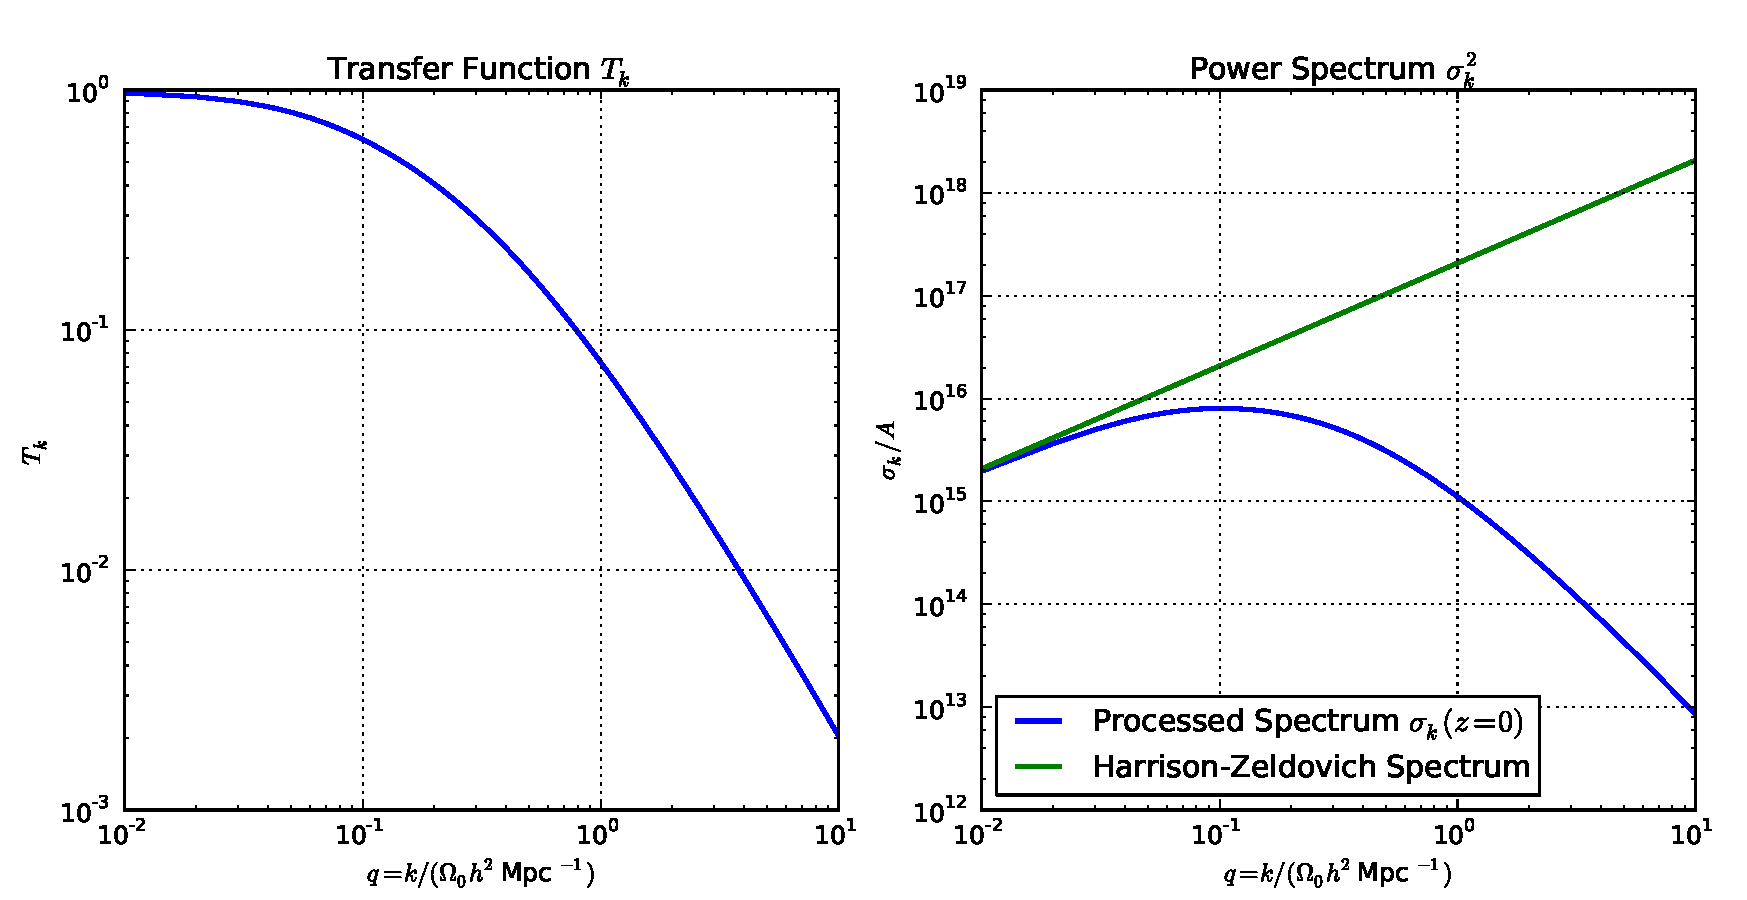
\includegraphics[width=0.9\textwidth]
	{./figures/2_theoretical_framework/Transfer_Function.pdf}

	\caption{\small{Función de transferencia para materia oscura fría en la
	época actual \cite{longair2008} (Izquierda). Comparación entre el 
	espectro de potencia inicial, Harrison-Zeldovich, y el espectro de 
	potencia procesado (derecha).}}
	
	\label{fig:TransferFunctionCDM}
\end{figure}
%.........................................................................	


De todo el formalismo desarrollado en esta sección se concluye que el 
objetivo final para la caracterización del régimen lineal es obtener la 
función de transferencia, ya que esta determina completamente la 
evolución del universo en épocas tempranas donde hay alta homogeneidad e
isotropía en todas las escalas.


%*************************************************************************




%*************************************************************************
%NonLinear Structure Formation
\section{Régimen No Lineal de Formación de Estructuras}
\label{sec:NonLinearStructureFormation}


En el régimen lineal se describe el proceso de formación de estructuras 
como perturbaciones en un universo de fondo homogéneo e isotrópico. Cuando
las perturbaciones crecen tal que $\delta \gtrsim 1$ la autogravedad de 
los modos acopla fuertemente el campo de forma local y e invalida la 
aproximación lineal. Los procesos físicos asociados al régimen no lineal
son altamente complejos e inclusive algunos no son bien entendidos en la 
actualidad, esto hace que solo sea posible abordar satisfactoriamente el 
problema a través de simulaciones numéricas (ver capítulo 
\ref{cha:N-BodySimulations}).


%.........................................................................
%Nonlinear Universe
\begin{figure}[htbp]
	\centering
	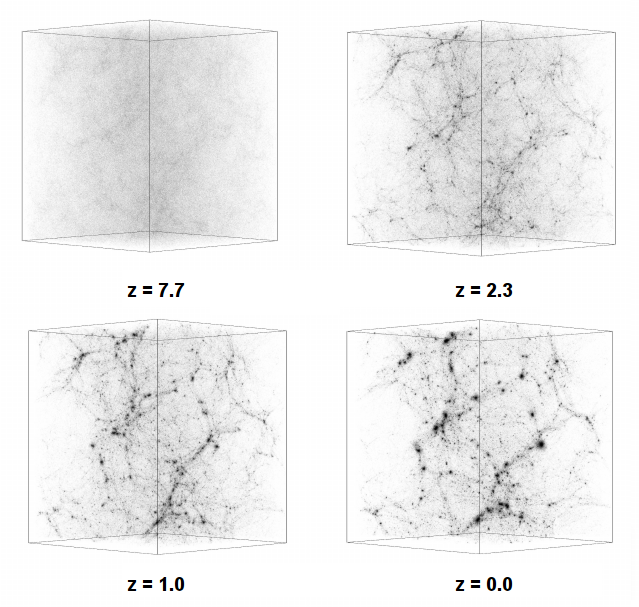
\includegraphics[width=0.9\textwidth]
	{./figures/2_theoretical_framework/Nonlinear.png}

	\caption{\small{Evolución de una simulación numérica de materia oscura
	en una caja de 40 Mpc$/h$, iniciando en un estado de alta homogeneidad 
	(arriba-izquierda) hasta la época actual de estructuras altamente no 
	lineales (abajo-derecha). Tomado de 
	\url{http://www.astro.utu.fi/research/CosmoS/lss/lss_p1.shtml}}}
	
	\label{fig:NonLinearUniverse}
\end{figure}
%.........................................................................


La figura \ref{fig:NonLinearUniverse} corresponde a una simulación 
numérica de materia oscura para el universo en régimen no lineal. En esta 
pueden ser apreciadas algunas propiedades emergentes tales como la 
anisotropía e inhomogeneidad a escalas peque\-ñas ($\sim$ Mpc), la 
formación y clustering de estructuras altamente no lineales y la aparición 
de un patrón de red a grandes escalas (red cósmica).


	%---------------------------------------------------------------------
	%Zeldovich's Approximation
	\subsection{Aproximación de Zeldovich}
	\label{subsec:Zeldovich'sApproximation}
	%---------------------------------------------------------------------
	

A pesar de la complejidad del régimen no lineal, cuando las perturbaciones 
en el campo de densidad aún no son mucho mayores que el valor de fondo 
puede realizarse una desarrollo analítico de la evolución, esto es conocido
como aproxi\-mación de Zeldovich y fue desarrollada en 1970 por Yakov 
Zeldovich en \cite{zeldovich1970}. Para formular esta aproximación es 
conveniente expresar de nuevo el campo de contraste de densidad 
$\delta(\bds r)$ en términos de coordenadas comóviles y no respecto a los 
modos normales de Fourier, esto debido a que en este régimen los modos no 
son independientes y usarlos no simplifica el tratamiento, a diferencia 
del régimen lineal. 


Usando el marco de referencia Lagrangiano de una cierta porción de fluido
o distribución de materia, su trayectoria $\bds r_f$ puede ser descrita 
mediante la siguiente expresión


%.........................................................................
\eq{eq:ZeldovichTrayectory}
{ \bds r_f( t,\bds q ) = a(t)\bds r = a(t)\cor{ \bds q + \bds \Psi(\bds q,t) } }
%.........................................................................
donde $\bds r$ es la posición comóvil de la porción de fluido, $\bds q$ 
su coordenada Lagrangiana inicial cuando el fluido no está perturbado y 
$\bds \Psi(\bds q,t)$ se denomina función de desplazamiento y da cuenta de 
las perturbaciones en el medio. 


A partir de la ecuación de evolución del campo de contraste de densidad 
\ref{eq:DeltaEvolution} es posible demostrar que el campo de desplazamiento 
$\bds \Psi(\bds q,t)$ satisface \cite{Yoshisato2006}


%.........................................................................
%Displacement Differential Equation
\eq{eq:Displacement}
{ \der{^2  \bds \Psi}{t^2} + 2H\der{\bds \Psi}{t} =
 \frac{ 3}{2}H^2 \bds \Psi  }
%.........................................................................
de esto se obtiene finalmente


%.........................................................................
%Displacement Explicit Form
\eq{eq:DisplacementForm}
{ \bds \Psi = \frac{3}{2}H_0^{-2}a(t)\nabla \Phi  }
%.........................................................................
donde $\Phi$ es el potencial gravitacional efectivo asociado al campo de 
densidad por medio de la ecuación de Poisson \ref{eq:PoissonEquationC}.


Expresando la conservación de la masa en términos de las coordenadas 
comóviles y las coordenadas Lagrangianas iniciales, se debe satisfacer


%.........................................................................
%Mass Conservation
\eq{eq:MassConservation}
{ \rho(\bds r, t)d^3 \bds r = \bar{\rho}(t)d^3 \bds q  }
%.........................................................................
calculando ahora el Jacobiano $\partial q_i / \partial r_j$ de la 
transformación $\bds r \rightarrow \bds q$, el campo de densidad perturbado 
pude se escrito como \cite{padmanabhan1995}


%.........................................................................
%Perturbed Field Density
\eq{eq:PerturbedFieldDensity}
{ \rho(\bds r, t) = \frac{\bar \rho (t)}{\pr{ 1 - a(t) \lambda_1(\bds q)}
\pr{ 1 - a(t) \lambda_2(\bds q)}\pr{ 1 - a(t) \lambda_3(\bds q)} } }
%.........................................................................
donde $-\lambda_i(\bds q)$ son los autovalores del Jacobiano y están 
ordenados de tal forma que $\lambda_1\geq\lambda_2\geq\lambda_3$. Cada uno
de estos autovalores pueden ser interpretados de forma geométrica como un 
indicador del colapso o expansión de una porción de fluido en la dirección
correspondiente al autovector respectivo, así por ejemplo si $\lambda_i > 0$,
implica que el campo de densidad está colapsando localmente en la dirección 
del autovector $\bds u_i$, mientras que $\lambda_i < 0$ implica una 
expansión en la misma dirección.

\
%.........................................................................
%Zeldovich Approximation Comparison
\begin{figure}[htbp]
	\centering
	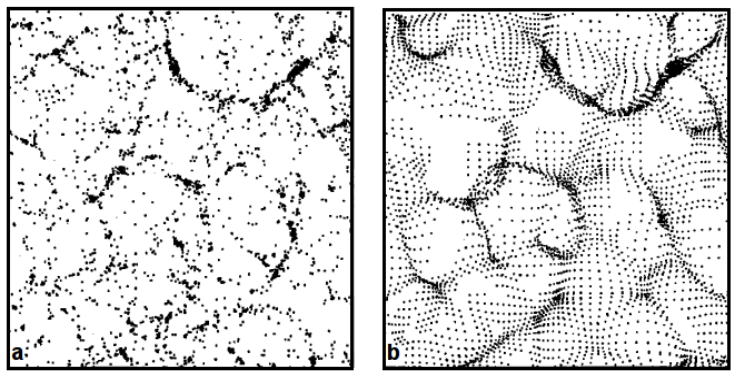
\includegraphics[width=0.9\textwidth]
	{./figures/2_theoretical_framework/Zeldovich_Approximation.png}

	\caption{\small{Comparación de la evolución en régimen no lineal entre
	una simulación de N-cuerpos (a), y la aproximación de Zeldovich (b).
	En ambos casos se usan las mismas condiciones iniciales. Tomado de 
	\cite{longair2008}. }}
	
	\label{fig:ZeldovichComparison}
\end{figure}
%.........................................................................


Finalmente en la figura \ref{fig:ZeldovichComparison} se muestra una 
comparación entre una simulación numérica de N-cuerpos y la aproximación 
de Zeldovich, puede notarse una alta semejanza visual en las estructuras 
obtenidas en los dos casos al final de la evolución, demostrando la alta 
precisión del método. En la sección \ref{sec:EnvironmentCharacterization}
se hace uso de la idea general planteada en la aproximación de Zeldovich 
respecto a los autovalores del Jacobiano de la transformación, para la 
construcción de esquemas de clasificación del entorno cosmológico a partir 
de los autovalores de otras cantidades físicas más adecuadas para la 
descripción de la dinámica local del campo de densidad, tales como el 
tensor de marea o el tensor de velocidad peculiar.


%*************************************************************************